\Section*{Introduction}

% pastille d'une limite (largeur fixe pour aligner les gloses) ; #1 : couleur, #2 : mot-clé
\newcommand{\limpill}[2]{\tikz[baseline=(n.base)]\node[draw=#1,text=#1,fill=white,rounded corners=3pt,inner sep=2pt,minimum width=2.1cm,font=\scriptsize](n){#2};}
% signe de la bulle : + (vert, contraste positif) ou − (rouge, limite), puis une glose très courte
\newcommand{\pro}[1]{\makebox[1.1em][l]{\textcolor{ForestGreen}{\textbf{+}}}#1}
\newcommand{\con}[1]{\makebox[1.1em][l]{\textcolor{darkred}{\textbf{$-$}}}#1}
% une ligne = la même bulle dans les deux cartes (critère), un signe et une glose ; #1 : overlays où la ligne est encadrée (orange), #2 : critère, #3 : \pro ou \con, #4 : glose
% toutes les lignes sont dans un cadre (sans trait ni fond si non mis en avant, de même encombrement) pour que l'alignement ne bouge pas
\newcommand{\crit}[4]{{\setlength{\fboxsep}{1pt}\setlength{\fboxrule}{0.8pt}%
			\alt<#1>{\fcolorbox{orange}{white}{\limpill{orange}{#2}\hspace{4pt}#3{\textcolor{orange}{#4}}}}%
			{\setlength{\fboxrule}{0pt}\setlength{\fboxsep}{1.8pt}\fbox{\limpill{neutral}{#2}\hspace{4pt}#3{#4}}}}\\[1pt]}
% carte d'une famille de méthodes : cadre contribbox du thème en neutre (le cadre des contributions est bleu / vert)
\newcommand{\methodcard}[2]{\begin{minipage}[t]{0.495\linewidth}\vspace{0pt}\begin{contribbox}{neutral}{#1}#2\end{contribbox}\end{minipage}}

\begin{frame}{Context and motivation}
	\textbf{Many-query contexts:} real-time simulation, digital twins, optimization, uncertainty quantification

	\vspace{3pt}
	$\Rightarrow$ \textbf{Goal:} solve a parametric PDE \coloredonly<1>{accurately} and \coloredonly<1>{quickly}, for many parameters $\bm{\mu}$

	\vspace{6pt}
	\only<2->{%
		\methodcard{Classical methods \footnotesize (FEM, FV, FD, spectral)}{%
			\crit{4-}{guarantees}{\pro}{error analysis}
			\crit{0}{single solve}{\pro}{efficient}
			\crit{0}{geometry}{\con}{mesh generation}
			\crit{0}{many queries}{\con}{one solve per $\bm{\mu}$}
			\crit{0}{expressivity}{\con}{fixed spaces}
		}
	} \hfill \only<3->{%
		\methodcard{Neural networks \footnotesize (PINN, neural operator)}{%
			\crit{0}{guarantees}{\con}{none}
			\crit{0}{single solve}{\con}{costly training}
			\crit{0}{geometry}{\pro}{mesh-free}
			\crit{0}{many queries}{\pro}{parametric}
			\crit{4-}{expressivity}{\pro}{flexible}
		}
	}

	\vspace{4pt}
	\only<4->{%
		\makebox[\linewidth][c]{\fcolorbox{orange}{white}{\textbf{\textcolor{orange}{Goal: classical guarantees + neural expressivity}}}}
	}

	% \vspace{3pt}
	% \only<5->{%
	% 	\makebox[\linewidth][c]{Existing enrichments are \coloredonly<5>{problem-dependent} $\Rightarrow$ two hybridizations: classical structure + neural expressivity}
	% }
\end{frame}
% \note{Petite note pour tester.}

% référence dans le corps de la slide (slide de biblio) : #1 clé, #2 auteurs abrégés (« et al. ») ; l'année est un lien vers la référence
\newcommand{\refin}[2]{{\footnotesize[#2, \citeyear{#1}]}}

\begin{frame}{Enriching the approximation space}
	\blk{1}{%
		\textbf{Hand-crafted bases:} GFEM \refin{StrouboulisCoppsBabuska2001}{Strouboulis et al.}, XFEM \refin{Moes1999}{Moës et al.}, Trefftz \refin{MoiolaPerugia2018}{Moiola and Perugia}
	}

	\vspace{6pt}
	\blk{2}{%
		$\Rightarrow$ \coloredonly<2>{problem-dependent}
	}

	\vspace{6pt}
	\blk{3}{%
		\textbf{Geometric prior:} $\varphi$-FEM \refin{DuprezLozinski2020}{Duprez and Lozinski}, \; $u = \varphi\, w$
	}

	\vspace{6pt}
	\blk*{4}{%
		\textbf{Neural prior:} learned level-set \refin{WanLiZha2025}{Wang et al.}, learned solution \refin{Franck2024}{Franck et al.}
	}

	\vspace{10pt}
	\only<5->{%
		\makebox[\linewidth][c]{\fcolorbox{orange}{white}{\textbf{\textcolor{orange}{Ours: classical method $+$ neural prior, two hybridizations}}}}
	}
\end{frame}

% hauteur commune des deux cartes d'hybridation (sinon elles suivent leur contenu)
\newcommand{\hybcardh}{5.1cm}

\begin{frame}{Two hybridizations}
	How does the \coloredonly<1>{neural network} enter the approximation space of a classical method?

	\vspace{6pt}
	\only<2->{%
		\begin{minipage}[t]{0.495\linewidth}\vspace{0pt}
			\tcbset{height=\hybcardh}\begin{contribbox}{cblue}{1st hybridization}
				\textbf{Enriched FEM using PINNs}

				\vspace{4pt}
				\centering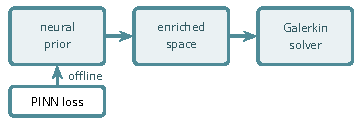
\includegraphics[page=1]{images/common/outline/outline.pdf}

				\vspace{4pt}
				\raggedright \textbf{Network:} pretrained, frozen\\[2pt]
				\textbf{Guarantees:} a priori error estimates
			\end{contribbox}
		\end{minipage}
	} \hfill \only<3->{%
		\begin{minipage}[t]{0.495\linewidth}\vspace{0pt}
			\tcbset{height=\hybcardh}\begin{contribbox}{cgreen}{2nd hybridization}
				\textbf{Learnable Galerkin methods\vphantom{g}}

				\vspace{4pt}
				\centering\includegraphics[page=2]{images/common/outline/outline.pdf}

				\vspace{4pt}
				\raggedright \textbf{Network:} learned through the solver\\[2pt]
				\textbf{Guarantees:} none (experimental)
			\end{contribbox}
		\end{minipage}
	}
\end{frame}

\begin{frame}{Parametric elliptic PDEs}
	Let $\Omega \subset \mathbb{R}^d$ be the spatial domain ($d=1,2,3$) and $\mathcal{M} \subset \mathbb{R}^p$ the parameter space.

	For one or several $\bm{\mu}\in \mathcal{M}$, find $u(\,\cdot\,;\bm{\mu}): \Omega\to \mathbb{R}$ such that

	\begin{equation}\label{eq:pde}\tag{$\mathcal{P}$}
		\left\{
		\begin{aligned}
			 & \mathcal{L}\big(u\,;\bm{x},\bm{\mu}\big) = f(\bm{x},\bm{\mu}), \; &  & (\bm{x},\bm{\mu}) \in \Omega \times \mathcal{M}, \\
			 & \text{Dirichlet, Neumann or Robin BC}, \;                         &  & (\bm{x},\bm{\mu}) \in \Gamma \times \mathcal{M},
		\end{aligned}
		\right.
	\end{equation}

	with $\Gamma:=\partial \Omega$ the boundary of $\Omega$,	$f$ the source term and $\mathcal{L}$ the linear differential operator defined by

	\begin{equation*}
		\mathcal{L}(\cdot\,;\bm{x},\bm{\mu}) : u \mapsto R(\bm{x},\bm{\mu})\, u + \bm{C}(\bm{x},\bm{\mu}) \cdot \nabla u - \frac{1}{\text{Pe}} \nabla \cdot \big(D(\bm{x},\bm{\mu}) \nabla u\big).
	\end{equation*}

	where $R$ is the reaction, $\bm{C}$ the convection, $D$ the (symmetric positive definite) diffusion matrix and $\text{Pe}$ the Péclet number.
\end{frame}
